% Options for packages loaded elsewhere
\PassOptionsToPackage{unicode}{hyperref}
\PassOptionsToPackage{hyphens}{url}
%
\documentclass[
]{article}
\usepackage{amsmath,amssymb}
\usepackage{lmodern}
\usepackage{iftex}
\ifPDFTeX
  \usepackage[T1]{fontenc}
  \usepackage[utf8]{inputenc}
  \usepackage{textcomp} % provide euro and other symbols
\else % if luatex or xetex
  \usepackage{unicode-math}
  \defaultfontfeatures{Scale=MatchLowercase}
  \defaultfontfeatures[\rmfamily]{Ligatures=TeX,Scale=1}
\fi
% Use upquote if available, for straight quotes in verbatim environments
\IfFileExists{upquote.sty}{\usepackage{upquote}}{}
\IfFileExists{microtype.sty}{% use microtype if available
  \usepackage[]{microtype}
  \UseMicrotypeSet[protrusion]{basicmath} % disable protrusion for tt fonts
}{}
\makeatletter
\@ifundefined{KOMAClassName}{% if non-KOMA class
  \IfFileExists{parskip.sty}{%
    \usepackage{parskip}
  }{% else
    \setlength{\parindent}{0pt}
    \setlength{\parskip}{6pt plus 2pt minus 1pt}}
}{% if KOMA class
  \KOMAoptions{parskip=half}}
\makeatother
\usepackage{xcolor}
\usepackage[margin=1in]{geometry}
\usepackage{color}
\usepackage{fancyvrb}
\newcommand{\VerbBar}{|}
\newcommand{\VERB}{\Verb[commandchars=\\\{\}]}
\DefineVerbatimEnvironment{Highlighting}{Verbatim}{commandchars=\\\{\}}
% Add ',fontsize=\small' for more characters per line
\usepackage{framed}
\definecolor{shadecolor}{RGB}{248,248,248}
\newenvironment{Shaded}{\begin{snugshade}}{\end{snugshade}}
\newcommand{\AlertTok}[1]{\textcolor[rgb]{0.94,0.16,0.16}{#1}}
\newcommand{\AnnotationTok}[1]{\textcolor[rgb]{0.56,0.35,0.01}{\textbf{\textit{#1}}}}
\newcommand{\AttributeTok}[1]{\textcolor[rgb]{0.77,0.63,0.00}{#1}}
\newcommand{\BaseNTok}[1]{\textcolor[rgb]{0.00,0.00,0.81}{#1}}
\newcommand{\BuiltInTok}[1]{#1}
\newcommand{\CharTok}[1]{\textcolor[rgb]{0.31,0.60,0.02}{#1}}
\newcommand{\CommentTok}[1]{\textcolor[rgb]{0.56,0.35,0.01}{\textit{#1}}}
\newcommand{\CommentVarTok}[1]{\textcolor[rgb]{0.56,0.35,0.01}{\textbf{\textit{#1}}}}
\newcommand{\ConstantTok}[1]{\textcolor[rgb]{0.00,0.00,0.00}{#1}}
\newcommand{\ControlFlowTok}[1]{\textcolor[rgb]{0.13,0.29,0.53}{\textbf{#1}}}
\newcommand{\DataTypeTok}[1]{\textcolor[rgb]{0.13,0.29,0.53}{#1}}
\newcommand{\DecValTok}[1]{\textcolor[rgb]{0.00,0.00,0.81}{#1}}
\newcommand{\DocumentationTok}[1]{\textcolor[rgb]{0.56,0.35,0.01}{\textbf{\textit{#1}}}}
\newcommand{\ErrorTok}[1]{\textcolor[rgb]{0.64,0.00,0.00}{\textbf{#1}}}
\newcommand{\ExtensionTok}[1]{#1}
\newcommand{\FloatTok}[1]{\textcolor[rgb]{0.00,0.00,0.81}{#1}}
\newcommand{\FunctionTok}[1]{\textcolor[rgb]{0.00,0.00,0.00}{#1}}
\newcommand{\ImportTok}[1]{#1}
\newcommand{\InformationTok}[1]{\textcolor[rgb]{0.56,0.35,0.01}{\textbf{\textit{#1}}}}
\newcommand{\KeywordTok}[1]{\textcolor[rgb]{0.13,0.29,0.53}{\textbf{#1}}}
\newcommand{\NormalTok}[1]{#1}
\newcommand{\OperatorTok}[1]{\textcolor[rgb]{0.81,0.36,0.00}{\textbf{#1}}}
\newcommand{\OtherTok}[1]{\textcolor[rgb]{0.56,0.35,0.01}{#1}}
\newcommand{\PreprocessorTok}[1]{\textcolor[rgb]{0.56,0.35,0.01}{\textit{#1}}}
\newcommand{\RegionMarkerTok}[1]{#1}
\newcommand{\SpecialCharTok}[1]{\textcolor[rgb]{0.00,0.00,0.00}{#1}}
\newcommand{\SpecialStringTok}[1]{\textcolor[rgb]{0.31,0.60,0.02}{#1}}
\newcommand{\StringTok}[1]{\textcolor[rgb]{0.31,0.60,0.02}{#1}}
\newcommand{\VariableTok}[1]{\textcolor[rgb]{0.00,0.00,0.00}{#1}}
\newcommand{\VerbatimStringTok}[1]{\textcolor[rgb]{0.31,0.60,0.02}{#1}}
\newcommand{\WarningTok}[1]{\textcolor[rgb]{0.56,0.35,0.01}{\textbf{\textit{#1}}}}
\usepackage{graphicx}
\makeatletter
\def\maxwidth{\ifdim\Gin@nat@width>\linewidth\linewidth\else\Gin@nat@width\fi}
\def\maxheight{\ifdim\Gin@nat@height>\textheight\textheight\else\Gin@nat@height\fi}
\makeatother
% Scale images if necessary, so that they will not overflow the page
% margins by default, and it is still possible to overwrite the defaults
% using explicit options in \includegraphics[width, height, ...]{}
\setkeys{Gin}{width=\maxwidth,height=\maxheight,keepaspectratio}
% Set default figure placement to htbp
\makeatletter
\def\fps@figure{htbp}
\makeatother
\setlength{\emergencystretch}{3em} % prevent overfull lines
\providecommand{\tightlist}{%
  \setlength{\itemsep}{0pt}\setlength{\parskip}{0pt}}
\setcounter{secnumdepth}{-\maxdimen} % remove section numbering
\ifLuaTeX
  \usepackage{selnolig}  % disable illegal ligatures
\fi
\IfFileExists{bookmark.sty}{\usepackage{bookmark}}{\usepackage{hyperref}}
\IfFileExists{xurl.sty}{\usepackage{xurl}}{} % add URL line breaks if available
\urlstyle{same} % disable monospaced font for URLs
\hypersetup{
  pdftitle={Stat 245 -- Test 2},
  pdfauthor={A. Student},
  hidelinks,
  pdfcreator={LaTeX via pandoc}}

\title{Stat 245 -- Test 2}
\author{A. Student}
\date{November 07, 2022}

\begin{document}
\maketitle

\#\#\#reading in Data-set

\begin{Shaded}
\begin{Highlighting}[]
\NormalTok{data1 }\OtherTok{\textless{}{-}} \FunctionTok{read.csv}\NormalTok{(}\StringTok{"https://sldr.netlify.app/data/sustainable{-}livelihoods.csv"}\NormalTok{)}\SpecialCharTok{|\textgreater{}}
  \FunctionTok{drop\_na}\NormalTok{(Increased\_Yield) }\SpecialCharTok{|\textgreater{}}
  \FunctionTok{drop\_na}\NormalTok{(Increased\_Knowledge)}\SpecialCharTok{|\textgreater{}}
  \FunctionTok{drop\_na}\NormalTok{(Food\_Ran\_Out)}
\end{Highlighting}
\end{Shaded}

\hypertarget{question-causual-diagram}{%
\subsubsection{question + causual
diagram}\label{question-causual-diagram}}

question: do the programs affect the individual's intellectuality and
yield where it makes sure that there is less food deprivation occurring
more often. (is there a association between food\_ran\_out and
increased\_knowledge and increased\_yield?)

\begin{figure}
\centering
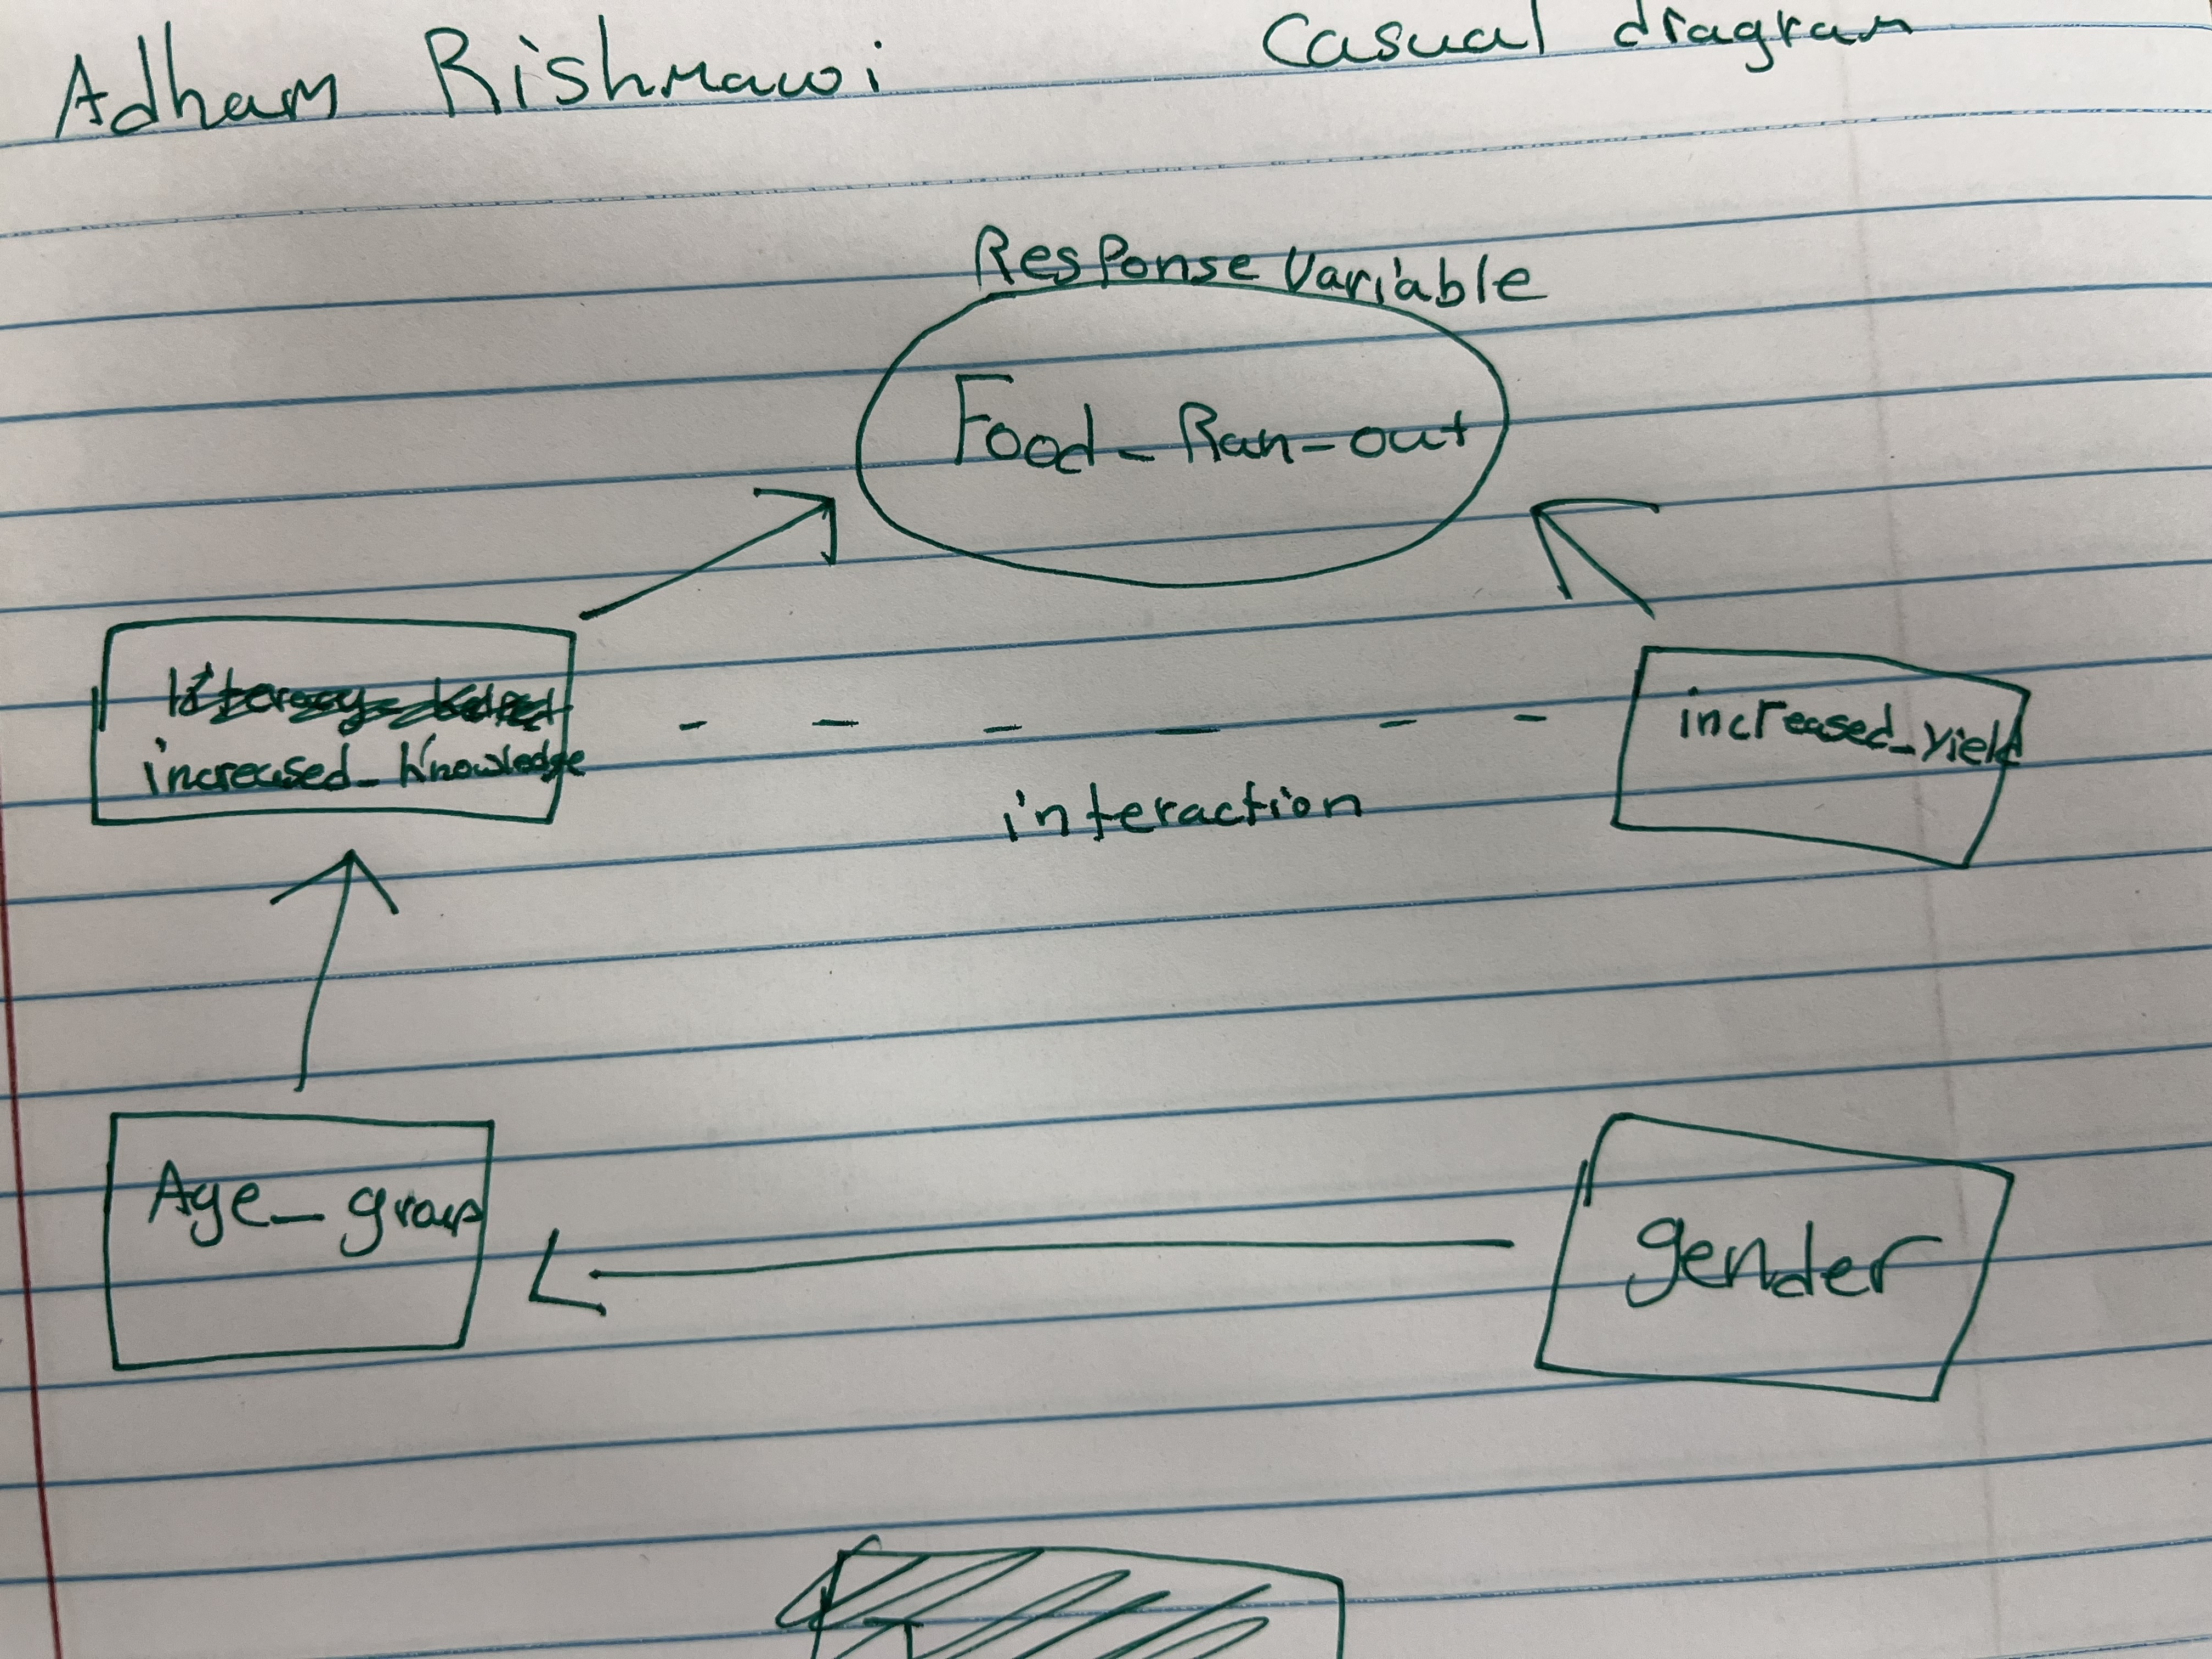
\includegraphics{cas_diag.jpg}
\caption{Casual Diagram}
\end{figure}

\#\#\#Justification for predictors and responses

Response variable: the reason I choose Food\_Ran\_Out is because I want
to do binary evaluation because this variable is either no or yes. I had
other options such as Months\_insufficient\_Food but I thought this
response variable would be more suitable because it is wthether they
completely ran out or not which is more simpler.

Predictors: -Increased\_knowledge \& increase\_yield: this i thought
would be a great predictor to pair up with increase\_yield because they
are both are binary options which we can study instances where both are
either 1 or zeros and see how they influence my response variable.
-Age-group: this an additional predictor that i thought would influence
my response variable because certain ages might be a contributor to the
reason why they ran out of food so i included it. -gender: This was a
given because I believed that due to cultural aspects and circumstances
that the reason why people would run out of food would be heavily based
on their gender. - the reason for the exclusion of other predictors: I
wanted to stay within the rule of thumb for this test and make sure that
my predictors did not go beyond this threshold. Other predictors would
have played into distorting the correlation between my response variable
and predictors.

\hypertarget{inital-graphs}{%
\subsubsection{Inital Graphs}\label{inital-graphs}}

\begin{Shaded}
\begin{Highlighting}[]
\NormalTok{int\_graph1 }\OtherTok{\textless{}{-}} \FunctionTok{gf\_boxplot}\NormalTok{(Food\_Ran\_Out }\SpecialCharTok{\textasciitilde{}}\NormalTok{ Increased\_Knowledge }\SpecialCharTok{|}\NormalTok{ Increased\_Yield ,  }\AttributeTok{data =}\NormalTok{ data1) }\SpecialCharTok{\%\textgreater{}\%}
  \FunctionTok{gf\_jitter}\NormalTok{(}\AttributeTok{alpha =} \FloatTok{0.3}\NormalTok{, }\AttributeTok{width =} \FloatTok{0.2}\NormalTok{) }\SpecialCharTok{\%\textgreater{}\%}
   \FunctionTok{gf\_labs}\NormalTok{(}\AttributeTok{subtitle =} \StringTok{"Initial graph elaborating assiocation between knowledge and the decrease of no food"}\NormalTok{,}
          \AttributeTok{title =} \StringTok{"Assiocation Graph for interaction"}\NormalTok{,}
          \AttributeTok{x =} \StringTok{" Increase of Knowledge"}\NormalTok{,}
          \AttributeTok{y =} \StringTok{"Did they have food?"}\NormalTok{, }
\NormalTok{           )}

\NormalTok{int\_graph1}
\end{Highlighting}
\end{Shaded}

\includegraphics{Test2_files/figure-latex/unnamed-chunk-2-1.pdf}

\begin{Shaded}
\begin{Highlighting}[]
\NormalTok{int\_graph2 }\OtherTok{\textless{}{-}} \FunctionTok{gf\_boxplot}\NormalTok{(Food\_Ran\_Out }\SpecialCharTok{\textasciitilde{}}\NormalTok{ Increased\_Yield }\SpecialCharTok{|}\NormalTok{ Increased\_Knowledge ,  }\AttributeTok{data =}\NormalTok{ data1) }\SpecialCharTok{\%\textgreater{}\%}
  \FunctionTok{gf\_jitter}\NormalTok{(}\AttributeTok{alpha =} \FloatTok{0.3}\NormalTok{, }\AttributeTok{width =} \FloatTok{0.2}\NormalTok{) }\SpecialCharTok{\%\textgreater{}\%}
   \FunctionTok{gf\_labs}\NormalTok{(}\AttributeTok{subtitle =} \StringTok{"Initial graph elaborating assiocation between Yield and the decrease of no food"}\NormalTok{,}
          \AttributeTok{title =} \StringTok{"Assiocation Graph for interaction"}\NormalTok{,}
          \AttributeTok{x =} \StringTok{" Increase of Food yield"}\NormalTok{,}
          \AttributeTok{y =} \StringTok{"Did they have food?"}\NormalTok{, }
\NormalTok{           )}

\NormalTok{int\_graph2}
\end{Highlighting}
\end{Shaded}

\includegraphics{Test2_files/figure-latex/unnamed-chunk-3-1.pdf}

\#\#\#Graph explanation Returning to the question we have in mind : do
the programs affect the individual's intellectuality and yield where it
makes sure that there is less food deprivation occurring more often.
ANSWER: Most definitely yes because we can observe an increase or a
difference in the amount of people who had food and did/didnt take the
program. I believe this makes my research question a topic worth going
into and evaluating. We could conclude hesitantly so far that the
programs have caused an increase in knowledge and yield which has caused
a decrease in the amount of food deprived people.

\hypertarget{fitting-regression-model}{%
\subsubsection{fitting regression
model}\label{fitting-regression-model}}

\begin{Shaded}
\begin{Highlighting}[]
\NormalTok{model\_fit }\OtherTok{\textless{}{-}} \FunctionTok{glmmTMB}\NormalTok{(}\FunctionTok{factor}\NormalTok{(Food\_Ran\_Out) }\SpecialCharTok{\textasciitilde{}}\NormalTok{ Increased\_Knowledge}\SpecialCharTok{*}\NormalTok{Increased\_Yield }\SpecialCharTok{+}\NormalTok{ Age\_Group }\SpecialCharTok{+}\NormalTok{ Gender, }
                 \AttributeTok{data =}\NormalTok{ data1, }
                 \AttributeTok{family =} \FunctionTok{binomial}\NormalTok{(}\AttributeTok{link =} \StringTok{\textquotesingle{}logit\textquotesingle{}}\NormalTok{))}


\FunctionTok{msummary}\NormalTok{(model\_fit)}
\end{Highlighting}
\end{Shaded}

\begin{verbatim}
##  Family: binomial  ( logit )
## Formula:          
## factor(Food_Ran_Out) ~ Increased_Knowledge * Increased_Yield +  
##     Age_Group + Gender
## Data: data1
## 
##      AIC      BIC   logLik deviance df.resid 
##    263.4    286.1   -124.7    249.4      181 
## 
## 
## Conditional model:
##                                     Estimate Std. Error z value Pr(>|z|)  
## (Intercept)                          -0.0341     0.7067  -0.048   0.9615  
## Increased_Knowledge                  -0.3604     0.9338  -0.386   0.6995  
## Increased_Yield                      -0.2099     0.7251  -0.290   0.7721  
## Age_Group50_plus                     -0.7289     0.3605  -2.022   0.0432 *
## Age_Groupunder_30                    -0.6324     0.4179  -1.513   0.1302  
## Gendermale                            0.2165     0.3029   0.715   0.4747  
## Increased_Knowledge:Increased_Yield   0.7334     0.9887   0.742   0.4582  
## ---
## Signif. codes:  0 '***' 0.001 '**' 0.01 '*' 0.05 '.' 0.1 ' ' 1
\end{verbatim}

\hypertarget{rationale-for-binary-and-logit}{%
\subsubsection{rationale for binary and
Logit}\label{rationale-for-binary-and-logit}}

1.The reasoning for selecting binary is because my response variable is
either 0(No)or 1 (yes) which makes it a great candidate for binary
regression model. 2.the reasoning for using model family logit is
because it was what Professor Ruiter suggested we use because a. it is
what the rest of the code we studied was in. b. it had the best average
between cloglog and probit.

\hypertarget{model-explanation}{%
\subsubsection{model explanation}\label{model-explanation}}

logit(p)=log(p/(1−pi))= beta0 + beta1IFood\_deprived + beta1IGender

parameters: n = number of trials p = probabilty of success

(pi/1-pi) = is the odds of success log = link function b2x2 + bGxG =
number of predictors

\#\#\#Assesments

\begin{Shaded}
\begin{Highlighting}[]
\NormalTok{s245}\SpecialCharTok{::}\FunctionTok{gf\_acf}\NormalTok{(}\SpecialCharTok{\textasciitilde{}}\NormalTok{model\_fit)}\SpecialCharTok{|\textgreater{}}
\FunctionTok{gf\_lims}\NormalTok{(}\AttributeTok{y=}\FunctionTok{c}\NormalTok{(}\SpecialCharTok{{-}}\DecValTok{1}\NormalTok{,}\DecValTok{1}\NormalTok{))}\SpecialCharTok{|\textgreater{}}
   \FunctionTok{gf\_labs}\NormalTok{(}\AttributeTok{subtitle =} \StringTok{"Assement1"}\NormalTok{, }\AttributeTok{title =} \StringTok{"Independence Of Residuals"}\NormalTok{, )}
\end{Highlighting}
\end{Shaded}

\includegraphics{Test2_files/figure-latex/unnamed-chunk-5-1.pdf}

This not good because the lines exceed the dashed lines which means this
residual ACf test failed! (issue with indepdence)

\begin{Shaded}
\begin{Highlighting}[]
\FunctionTok{require}\NormalTok{(DHARMa)}
\NormalTok{food\_sim }\OtherTok{\textless{}{-}} \FunctionTok{simulateResiduals}\NormalTok{(model\_fit)}

\FunctionTok{gf\_point}\NormalTok{(food\_sim}\SpecialCharTok{$}\NormalTok{scaledResiduals }\SpecialCharTok{\textasciitilde{}} \FunctionTok{rank}\NormalTok{(}\FunctionTok{predict}\NormalTok{(model\_fit)),}
         \AttributeTok{alpha =} \FloatTok{0.2}\NormalTok{) }\SpecialCharTok{|\textgreater{}}
  \FunctionTok{gf\_labs}\NormalTok{(}\AttributeTok{x =} \StringTok{\textquotesingle{}Fitted Values\textquotesingle{}}\NormalTok{,}
          \AttributeTok{y =} \StringTok{\textquotesingle{}Scaled Residuals\textquotesingle{}}\NormalTok{)}
\end{Highlighting}
\end{Shaded}

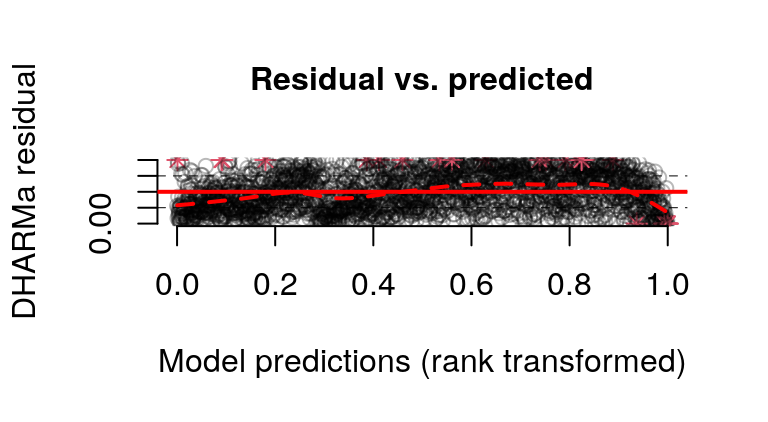
\includegraphics{Test2_files/figure-latex/unnamed-chunk-6-1.pdf}

This absolutely failed the test because a. it is not universally
distributed which is the main case. the mean-variance relationship is
severely bad here!!!

\begin{itemize}
\tightlist
\item
  after some re-evaluating I can say that this graph is borderline
  passable because of the uniformately starting from the top right
  corner! but the left corner concerns me so i would still stick to my
  initial statement.
\end{itemize}

\hypertarget{selection}{%
\subsubsection{Selection}\label{selection}}

\begin{Shaded}
\begin{Highlighting}[]
\NormalTok{car}\SpecialCharTok{::}\FunctionTok{Anova}\NormalTok{(model\_fit)}
\end{Highlighting}
\end{Shaded}

\begin{verbatim}
## Analysis of Deviance Table (Type II Wald chisquare tests)
## 
## Response: factor(Food_Ran_Out)
##                                      Chisq Df Pr(>Chisq)  
## Increased_Knowledge                 0.9414  1    0.33191  
## Increased_Yield                     0.1411  1    0.70718  
## Age_Group                           5.1246  2    0.07713 .
## Gender                              0.5111  1    0.47467  
## Increased_Knowledge:Increased_Yield 0.5503  1    0.45821  
## ---
## Signif. codes:  0 '***' 0.001 '**' 0.01 '*' 0.05 '.' 0.1 ' ' 1
\end{verbatim}

This is not good\ldots{} We can observe here that there is any
indication that there are strong predictors to Food\_Ran\_out. The best
extraction from this Anova is that the best predictor to this prediction
plot is Age\_Group which makes some sense. It is even hard to determine
that there any interaction going on here through the Pr so I am
concerned and know that these predictors dont play into altering
food\_Ran\_Out.

\#\#\#shortcut pred plot because there is no assiocation between the two

\begin{Shaded}
\begin{Highlighting}[]
\NormalTok{pre\_preds }\OtherTok{\textless{}{-}}\NormalTok{ ggeffects}\SpecialCharTok{::}\FunctionTok{ggpredict}\NormalTok{(model\_fit, }\FunctionTok{c}\NormalTok{(}\StringTok{"Increased\_Knowledge"}\NormalTok{, }\StringTok{"Increased\_Yield"}\NormalTok{))}
\FunctionTok{plot}\NormalTok{(pre\_preds)}
\end{Highlighting}
\end{Shaded}

\includegraphics{Test2_files/figure-latex/unnamed-chunk-8-1.pdf}

This is exactly what I expected because I concluded that there is no
association between the two variables im evaluating in model assessments
and this graph reassures this statement. Here we observed that the red
shaded area is within the blue which tells us that there is no
intersection hence no interaction!

\hypertarget{conclusion}{%
\subsubsection{Conclusion}\label{conclusion}}

restated research question: do the programs affect the individual's
intellectuality and yield where it makes sure that there is less food
deprivation occurring more often. (is there a association between
food\_ran\_out and increased\_knowledge/increased\_yield?)

answer based on initial graph: there was potential because we observed
plenty of queues which indicated to the user that there was some kind of
assiocation between the interaction I had in mind.

answer based on model assessment: this is where all my confidence was
shifted to the worst and I truly observed no association and plenty of
model assessments. both tests failed!

answer based on prediction plot: This graph served as the verification
for my selection and model assessment it's failure aligned with the
projection I had when I saw the results of the assessments.

answer based on model selection: instantly looking at the model
selection process we observed that no correlation or predictors were
influencing the response variable we had so I discovered that my initial
research question is proven wrong rather then right!!!

\end{document}
